\documentclass[../main/main.tex]{subfiles}

\makeatletter
\renewcommand{\@chapapp}{Optique -- chapitre}
\makeatother

\begin{document}

\chapter{Propagation de la lumi\`ere}

\section{L'onde lumineuse}

\subsection{Nature ondulatoire de la lumière}

La nature de la lumière a été l'objet de discussions et controverses durant des
siècles, opposant principalement au XVII\ieme\ \textsc{Newton} avec sa théorie
corpusculaire et \textsc{Hooke} puis \textsc{Huygens} avec la théorie
ondulatoire. Le débat s'est clos avec les expériences d'interférences de
\textsc{Young} et \textsc{Fresnel} (début XIX\ieme) notamment, prouvant son
comportement ondulatoire (nous aurons l'occasion de les réaliser nous-mêmes),
mais ce n'est qu'à la fin du XIX\ieme\ avec les théories de \textsc{Maxwell} que
cette onde est décrite par la propagation de grandeurs électromagnétiques (champ
électrique, champ magnétique, et donc pas dans un milieu matériel).

Le XX\ieme\ vint bousculer cette vision en attestant de la dualité
onde-corpuscule des particules élémentaires de l'Univers avec l'avènement de la
physique quantique. Selon les conditions d'études, l'une ou l'autre des visions
sera appliquée.

\subsection{Célérité de la lumière}

\subsubsection{Dans le vide}

En tant qu'onde électromagnétique, la lumière n'est pas une onde mécanique
nécessitant un milieu matériel pour se propager\footnote{À la différence d'une
    vague sur l'eau ou d'une corde de guitare qui se propagent sur un milieu
matériel.}.

\begin{tcbraster}[raster columns=5, raster equal height=rows]
    \begin{NCdefi}[raster multicolumn=2]{Définition}
        Nous appelons \textit{célérité} de la lumière \textbf{dans le vide}, et
        la notons $c$, la vitesse de l'onde lumineuse.
    \end{NCdefi}
    \begin{NCodgr}[raster multicolumn=3]{Valeur}
        La valeur de $c$ est fixée par définition\footnote{elle n'est donc
            théoriquement plus mesurable, puisque les mesures de distances se
        basent sur la valeur de la célérité de la lumière}, telle que
        \[c = \SI{2.99792458e8}{m.s^{-1}}\]
        Nous utiliserons et retiendrons cependant la valeur
        \[\boxed{c = \SI{3.00e8}{m.s^{-1}}}\]
    \end{NCodgr}
\end{tcbraster}

\subsubsection{Dans un milieu}

Elle peut cependant se propager dans certains milieux matériels transparents,
comme l'air, l'eau, le verre… Dans le cadre de la physique de cette année, nous
étudierons des milieux particuliers~:

\vfill

\begin{NCdefi}{Définition~: milieu transparent linéaire homogène isotrope (TLHI)}
    \begin{itemize}[leftmargin=66pt]
        \item[\textbf{Transparent}] : qui laisse passer la lumière~;
        \item[\textbf{Linéaire}] : dont les sorties sont proportionnelles aux
            entrées~;
        \item[\textbf{Homogène}] : dont les propriétés physiques sont
            constantes en tout point du milieu~;
        \item[\textbf{Isotrope}] : dont les propriétés physiques ne
            dépendent pas de la direction de la lumière dans le milieu.
    \end{itemize}
\end{NCdefi}

Lorsque la lumière passe dans un tel milieu, sa vitesse \textbf{diminue}. Nous
caractérisons cette diminution \textit{via} la définition de l'indice optique~:

\begin{tcbraster}[raster columns=3, raster equal height=rows]
    \begin{NCdefi}[raster multicolumn=2, sidebyside]{Définition~: indice optique}
        Nous appelons \textit{indice optique} la grandeur associée à milieu
        transparent et caractérisant la vitesse de la lumière en son sein, telle
        que~:

        \begin{empheq}[box=\fbox]{equation*}
            n = \frac{c}{v}
        \end{empheq}

        \tcblower
        \tcbsubtitle[before skip=\baselineskip,
                     colback=green!50!black,
                     colframe=green!50!black]{Unités}

        En tant que rapport de deux grandeurs de même unité, l'indice optique
        n'a pas d'unité.

    \end{NCdefi}
    \begin{NCrema}[]{Remarque}

        Étant donné que la vitesse de la lumière \textbf{dans le vide} est
        absolue et indépassable, la vitesse de la lumière dans un milieu
        transparent ne peut qu'être plus petite, et donc \textbf{l'indice
        optique est toujours > 1}.

    \end{NCrema}
\end{tcbraster}

\begin{tcbraster}[raster columns=4, raster equal height=rows]
    
    \begin{NCimpl}[]{Implication}
        Par la définition de l'indice optique, nous en déduisons évidemment~:
        \begin{empheq}[box=\fbox]{equation*}
            v = \frac{c}{n}
        \end{empheq}
    \end{NCimpl}
    \begin{NCodgr}[raster multicolumn=3]{Ordre de grandeur}
        \begin{tabularx}{\linewidth}{Y*{2}{Y}}
            \toprule
            Milieu  & $n$                  & $v [\si{m.s^{-1}}]$\\
            \midrule
            Vide    & 1                    & \num{3.00e8}\\
            Air     & $\approx$ \num{1.00} & \num{3.00e8}\\
            Eau     & \num{1.33}           & \num{2.3e8}\\
            Verre   & \num{1.5}            & \num{2.0e8}\\
            Diamant & \num{2.4}            & \num{1.25e8}\\
            \bottomrule
        \end{tabularx}
    \end{NCodgr}

\end{tcbraster}

\subsubsection{Selon la fréquence}

L'indice optique dépend de la fréquence d'une onde lumineuse, et ainsi la
vitesse de la lumière dans un milieu TLHI aussi. Comme la couleur de la lumière
correspond à la fréquence de l'onde la représentant, cela cause la
\textbf{dispersion} de la lumière\footnote{Pensez par exemple au prisme de Pink
Floyd.}. Cet effet est cependant souvent négligé car faible par rapport à
d'autres phénomènes.

\subsection{Longueur d'onde d'une onde sinusoïdale}

\begin{tcbraster}[raster columns=2, raster equal height=rows]
    
    \begin{NCdefi}[]{Définition~: onde sinusoïdale}

        Une onde sinusoïdale est une onde \textbf{monochromatique}, ce qui
        signifie «~une seule couleur~». Elle est donc décrite par une unique
        valeur de longueur d'onde ou de fréquence, et non pas comme une
        superposition.

    \end{NCdefi}
    \begin{NCexem}[]{Exemples}
    
        Une lumière rouge est monochromatique, et est décrite par une onde
        lumineuse de longueur d'onde $\approx \SI{700}{nm}$. Une lumière blanche
        ne l'est pas, c'est une superposition d'ondes sinusoïdales sur le
        domaine du visible.
    
    \end{NCexem}
\end{tcbraster}

\begin{tcbraster}[raster columns=3, raster equal height=rows]
    \begin{NCprop}[]{Propriété}

        Une onde lumineuse se caractérise par sa fréquence, appelée $f$ ou
        $\nu$\footnote{Se lit «~nu~».}. En effet, \textbf{la fréquence d'une
        onde est indépendante du milieu traversé}. En revanche, sa
        \textbf{longueur d'onde en dépend}.

    \end{NCprop}
    \begin{NCimpl}[raster multicolumn=2]{Implication}
        Avec l'analyse dimensionnelle, on trouve directement qu'une longueur
        d'onde $\lambda$ doit s'écrire

        \[\lambda = \frac{v_{\rm onde}}{f_{\rm onde}}\]
    
        Or, dans le vide $v_{\rm onde} = c$, et dans un milieu TLHI d'indice
        optique $n$, $v_{\rm onde} = \frac{c}{n}$~; ainsi avec $\lambda_0$ dans
        le vide~:
    
        \begin{equation*}
            \boxed{\lambda_0 = \frac{c}{f}}
            \quad\text{et}\quad
            \boxed{\lambda = \frac{c}{n\times f} = \frac{\lambda_0}{n}}
        \end{equation*}
    \end{NCimpl}
\end{tcbraster}

Ainsi, quand on parle de la longueur d'onde d'une couleur, on parle en réalité
de sa longueur d'onde \textit{dans le vide}.

\begin{figure}[h]
    \centering
    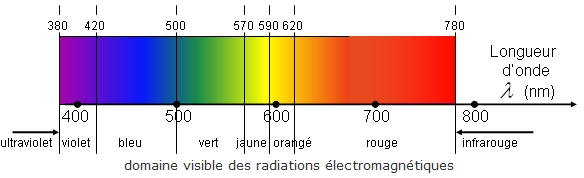
\includegraphics[width=\linewidth]{ch1_fig1.png}
    \captionsetup{justification=centering}
    \caption{Longueurs d'ondes des ondes monochromatiques dans le domaine
    visible et \textbf{dans le vide}.}
    \label{fig:lambda_vis}
\end{figure}

\begin{NCexem}[]{Exercice}
    Un laser rouge émet un rayonnement de longueur d'onde dans le vide
    $\lambda_0 = \SI{633}{nm}$. Déterminer sa longueur d'onde $\lambda$ dans du
    verre, d'indice optique $n = \num{1.5}$. Sa couleur change-t-elle~?
    \tcblower
    \vspace{2cm}
\end{NCexem}

\section{Sources lumineuses primaires}

On parle de source primaire quand l'objet en question émet directement de la
lumière. Les sources secondaires ne font qu'en renvoyer, par exemple la Lune, la
peau, les arbres…

\subsection{Spectre d'émission}

Pour caractériser un rayonnement électromagnétique, on trace son spectre
d'émission, c'est-à-dire la courbe de l'intensité lumineuse en fonction de la
fréquence (ou longueur d'onde dans le vide).

Les sources primaires sont classées selon leur contenu spectral
qui découle du type de processus d'émission lumineuse~:
\begin{itemize}[leftmargin=120pt]
    \item[\textbf{Sources thermiques}] : agitation thermique des atomes~;
    \item[\textbf{Sources spectrales}] : excitation électrique des atomes~;
    \item[\textbf{Sources LASER}] : optimisation de l'émission stimulée de photons.
\end{itemize}

\subsection{Les sources thermiques}

L'agitation thermique des atomes émet un rayonnement électromagnétique dépendant
de sa température~: c'est le type de rayonnement du Soleil ou des ampoules à
incandescence (chauffage d'un métal qui brille).

\begin{NCdefi}[]{Caractéristiques du rayonnement d'un corps chaud}
    Le spectre d'émission d'une source thermique est une courbe
    \textbf{continue}, étalée autour d'une longueur d'onde d'émission maximale
    $\lambda_{\max}$. Plus la température augmente, plus le spectre se déplace vers
    une fréquence élevée (ou longueur d'onde faible)~: une étoile bleue est bien
    plus chaude qu'une étoile rouge.
\end{NCdefi}

\begin{NCexem}[sidebyside]{Exemples}
    \begin{itemize}
        \item À température ambiante ($T \approx \SI{300}{K}$), un corps émet
            dans l'infrarouge (c'est le principe d'une caméra infrarouge)~;
        \item Pour une lampe, le filament est à $T \approx \SI{2800}{K}$. Son
            maximum est dans l'infrarouge mais son spectre s'étale sur le
            domaine visible~;
        \item La température de surface du Soleil est de $T \approx
            \SI{5700}{K}$. Son maximum d'émission est dans le domaine visible.
    \end{itemize}
    \tcblower
    \begin{center}
        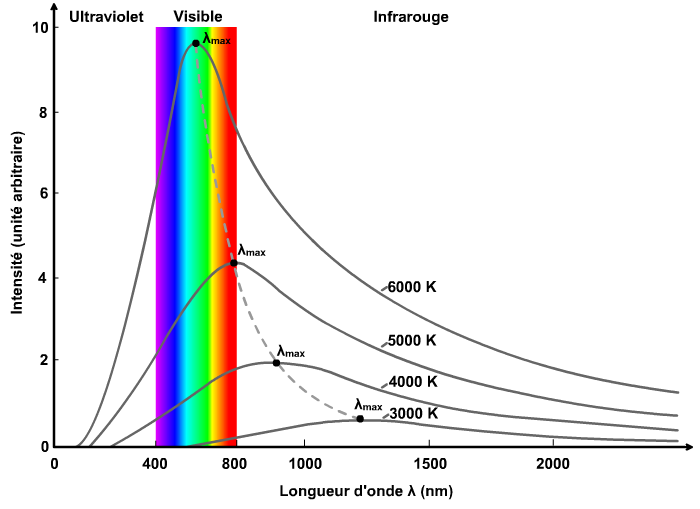
\includegraphics[width=\linewidth]{ch1_fig2.png}
        \captionof{figure}{Spectre d'émission d'un corps chaud selon quelques
        températures.}
        \label{fig:cps_chaud}
    \end{center}
\end{NCexem}

\subsection{Les sources spectrales}

Une lampe spectrale contient un élément chimique sous forme de gaz, et deux
électrodes de part et d'autre du contenant génère des décharges électriques qui
excitent les atomes. C'est un état instable. En revenant dans leur état
fondamental, ils émettent des photons à une énergie précise correspondant à la
différence des niveaux d'énergie quantiques de l'élément ($f = \frac{\Delta
E}{h}$~; voir chapitre introduction à la physique quantique).

\begin{NCdefi}[]{Caractéristiques du rayonnement spectral}
    Le spectre d'émission d'un rayonnement spectral est composé de pics
    d'intensités faiblement élargis. Les longueurs d'onde de ces pics sont
    caractéristiques de l'élément excité~; c'est de cette manière qu'on peut
    déterminer la composition atmosphérique des exoplanètes ou caractériser les
    étoiles.
\end{NCdefi}
\begin{NCexem}[sidebyside, righthand width=.5\linewidth]{Exemples}
    On trouve des lampes au néon, de couleur rouge~; des lampes au mercure, de
    couleur bleue~; des lampes à sodium, dans l'orange… On utilisera
    principalement ces deux dernières en laboratoire.
    \tcblower
    \begin{center}
        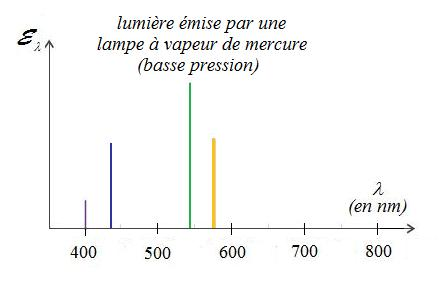
\includegraphics[width=.9\linewidth]{ch1_fig3.jpg}
        \captionof{figure}{Spectre d'émission d'une lampe à vapeur de mercure.}
        \label{fig:lamp_spec}
    \end{center}
\end{NCexem}

\subsection{Le LASER}
LASER est l'acronyme de \textit{Light Amplification by Stimulated Emission of
Radiations}, c'est-à-dire «~amplification de la lumière par émission stimulée de
radiations~». Il est composé d'une cavité remplie d'un milieu recevant de
l'énergie, excité par une source extérieur, et fermée par deux miroirs. Celui de
la face de sortie est légèrement transparent.

La lumière passe au travers du milieu qui réémet de la lumière sans atténuer la
première, et grâce au miroir le tout est réfléchi pour permettre de nombreux
aller-retours, amplifiant l'intensité lumineuse à chaque passage.

\begin{NCdefi}[]{Caractéristiques du rayonnement LASER}
    Le spectre du laser ne contient qu'une seule raie extrêmement fine, bien
    plus fine que celle des sources spectrales. C'est l'exemple le plus proche
    d'une réelle source monochromatique.
\end{NCdefi}
\begin{NCexem}[sidebyside]{Exemple}
    Un laser hélium-néon donne un faisceau rouge de longueur d'onde dans le vide
    $\lambda_0 = \SI{632.8}{nm}$.
    \tcblower
    \begin{center}
        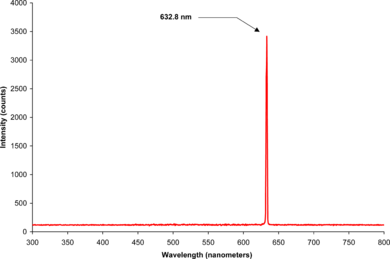
\includegraphics[width=.8\linewidth]{ch1_fig4.png}
        \captionof{figure}{Spectre d'émission d'un laser hélium-néon.}
        \label{fig:laser_spec}
    \end{center}
\end{NCexem}
\begin{NCimpo}[hand]{Attention}
    Si la puissance totale du faisceau est communément assez faible ($P \approx
    \SI{1}{mW}$), sa surface l'est également ($S \approx \SI{1}{mm^2}$). La
    puissance \textit{surfacique} est donc en réalité très grande, et
    particulièrement dangereuse pour l'œil. On veillera donc à ne jamais le
    diriger vers un œil, mais aussi à éviter toute réflexion involontaire
    (notamment sur tout métal~: bijou, tige de support…).
\end{NCimpo}

\section{Diffraction de la lumière}

\subsection{Principe}

La nature ondulatoire de la lumière apparaît clairement lors des expériences de
diffraction~: dans certains cas, la restriction d'un faisceau lumineux (par
exemple un laser) par une fente, donne sur un écran placé loin derrière, un
étalement de la lumière \textbf{plus large} que la largeur de la fente.

\begin{figure}[h]
    \centering
    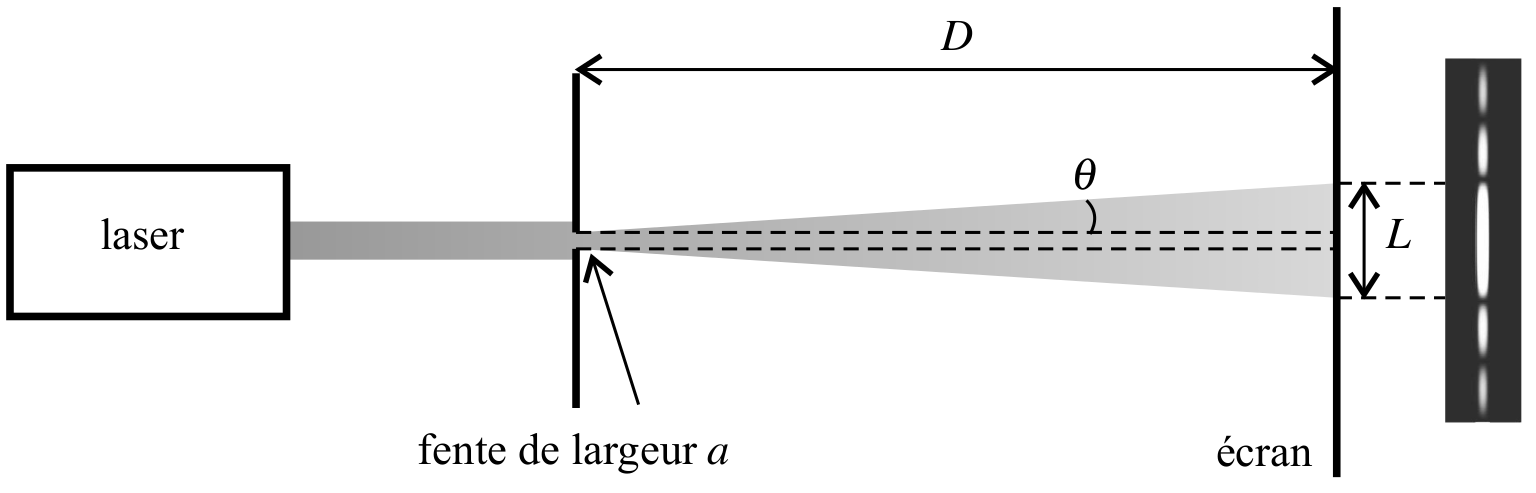
\includegraphics[width=.8\linewidth]{ch1_fig5}
    \captionsetup{justification=centering}
    \caption{Diffraction de \textsc{Fraunhofer} d'un faisceau laser par une
    fente fine.}
    \label{fig:diff_las}
\end{figure}

Ce phénomène survient quand l'extension spatiale d'une onde est limitée~; cela
arrive également avec les vagues dans l'eau. En effet, pour des valeurs de
largeur de fente $a \gg \lambda$, il n'y a bien qu'une coupure du faisceau. En
revanche, quand $a \approx \lambda$, ce phénomène survient. On observe même que
plus $a$ est petit, plus la lumière s'étale sur l'écran.

\subsection{Loi de la diffraction}

\begin{loi}[label=loi:diffraction]{diffraction par une fente simple}
    Un faisceau monochromatique de longueur d'onde $\lambda$ dans le vide,
    limité spatialement par une fente de largeur $a \approx \lambda$, forme à
    grande distance sur un écran des tâches lumineuses dont le demi angle
    d'ouverture $\theta$ de la tâche centrale vérifie
    \begin{empheq}[box=\fbox]{equation*}
        \sin(\theta) = \frac{\lambda}{a}
    \end{empheq}
\end{loi}

% \theendnotes

\end{document}
